\documentclass[fontsize=12pt]{scrartcl} % paper size, default font size
% \usepackage[T1]{fontenc} % Use 8-bit encoding that has 256 glyphs
% \usepackage{fourier} % Use the Adobe Utopia font for the document - comment this line to return to the LaTeX default
\usepackage[letterpaper, margin=1.0in]{geometry}
\usepackage[english]{babel} % English language/hyphenation
\usepackage{amsmath,amsfonts,amsthm,amssymb} % Math packages
\usepackage{times,graphicx,epstopdf,url,xspace, listings, enumitem,indentfirst} % assorted formatting
\usepackage{sectsty} % Allows customizing section commands
\usepackage{listings} % allows for code
\allsectionsfont{ \normalfont\scshape} %  the default font and small caps
% \centering
\usepackage{fancyhdr} % Custom headers and footers
\pagestyle{fancyplain} % Makes all pages in the document conform to the custom headers and footers
\fancyhead{} % No page header - if you want one, create it in the same way as the footers below
\fancyfoot[L]{Tekuma, Inc.} % Empty left footer
\fancyfoot[C]{} % Empty center footer
\fancyfoot[R]{\thepage} % Page numbering for right footer
\renewcommand{\headrulewidth}{0pt} % Remove header underlines
\renewcommand{\footrulewidth}{0pt} % Remove footer underlines
\setlength{\headheight}{13.6pt} % Customize the height of the header

\numberwithin{equation}{section} % Number equations within sections (i.e. 1.1, 1.2, 2.1, 2.2 instead of 1, 2, 3, 4)
\numberwithin{figure}{section} % Number figures within sections (i.e. 1.1, 1.2, 2.1, 2.2 instead of 1, 2, 3, 4)
\numberwithin{table}{section} % Number tables within sections (i.e. 1.1, 1.2, 2.1, 2.2 instead of 1, 2, 3, 4)

\setlength\parindent{26pt} % Removes all indentation from paragraphs - comment this line for an assignment with lots of text

%  Set the line spacing for the document here:
\usepackage{setspace}
% \doublespacing
% or:
\onehalfspacing

%----------------------------------------------------------------------------------------
%	TITLE SECTION
%----------------------------------------------------------------------------------------

\newcommand{\horrule}[1]{\rule{\linewidth}{#1}} % Create horizontal rule command with 1 argument of height

\title{
\normalfont \normalsize
\textsc{Tekuma, Inc} \\[6pt]
\horrule{0.2pt} \\[10pt] % Thin top horizontal rule
\Huge The Tekuma Art Curation System  % The assignment title
\horrule{1.5pt}  % Thick bottom horizontal rule
\normalsize \{stwhite,anyati\}@mit.edu
}
\author{\textbf{Stephen L. White and Afika Nyati}}
\date{\normalsize \today} % Today's date or a custom date

%-------------------------------------------------------------------------------

\begin{document}
\maketitle % Print the title

\section{Overview}
There has been approximately one year to date of active, ongoing technologies development at Tekuma, Inc. When development began in June 2016, very little web infrastructure existed besides the tekuma homepage\footnote{http://tekuma.io. A WordPress static website}. The first goal realized was to build a system for onboarding, cataloging, and accessing artworks in an effort to streamline the art curation process happening at Tekuma, and provide a more scalable business model. One year later, much of the infrastructure for this goal has been implemented, and is ready for innovative and more marketable applications to be built on top of this curation infrastructure. (give a total count of lines of code, components, etc)

\section{Components}
The infrastructure which would most help Tekuma’s curation process was not clear at the time development began. Design decisions were made as they arose, as Tekuma's needs and use cases were evolving with the development. Different prototypes were being tested to analyze different possible web technologies that could be used. After two weeks of prototyping, it became apparent that some preliminary specification needed to be defined in order to structure development of the core infrastructure and to drive production forward. In June 2016, Stephen decided that a four-sided approach would best meet the needs of Tekuma’s complex business model, and multiple targeted users. Specifically, an underlying cloud-based system serves 4 web apps to act as portals into different parts of Tekuma's curation system. These web apps are referred to as the ABCD user abstraction. This model is described below and summarized in figure (2.1), where each entry represents an online hosted application. All code connected to the curation system is stored in Tekuma's GitHub. \footnote{https://github.com/tekuma}

\begin{figure}
    \begin{tabular}{|l|l|l|l|l|}
    \hline
      & Name & Targeted Users & URL & Repository \\
    \hline
    \textbf{A} & The Artist Portal & Artists & https://artist.tekuma.io & artist-portal \\
    \hline
    \textbf{B} & The Business Portal & Property Owners & https://business.tekuma.io * & n/a \\
    \hline
    \textbf{C} & The Curator Portal & Curators & https://curator.tekuma.io & curator-portal \\
    \hline
    \textbf{D} & The Discover Portal & Consumers & https://discover.tekuma.io & n/a\\
    \hline
    \end{tabular}
    \caption{the ABCD User Abstraction}
    \label{label}
\end{figure}

\begin{figure}
    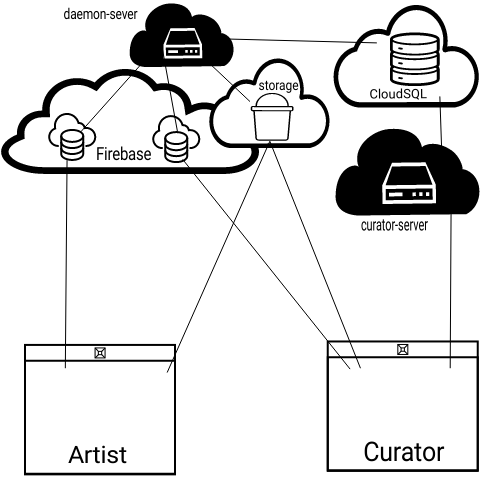
\includegraphics[scale=.5]{./img/tekuma-1}
    \caption{Arist-Curator System Diagram}
    \label{}
\end{figure}

\subsection{Boilerplate}
Before creating the web applications, a general boilerplate was designed for online user interfaces. The boilerplate makes up Tekuma’s online graphic and visual identity. The UI primarily defaults to customs and principles dictated by Google’s Material Design\footnote{ https://material.io/guidelines/ } in line with the current standards in User Interface design. Also included with the boilerplate is Tekuma’s general CSS stylesheet, and a set of interface icons created by Afika Nyati. The style sheet builds upon the material design guidelines by customizing it to Tekuma’s aesthetics. More technically, the interface is written in JavaScript ES6+ using ReactJS, transpiled using webpack and BabelJS. State in the interfaces, user account creation, and file uploads are all handled by Google Firebase and managed in the Firebase Conosole\footnote{}. For simplicity, all code in the system is written in JavaScript and is either executed in-browser, or with NodeJS (v6.4.0LTS). Together, the stylesheet, ReactJS interface components, logo, color palette and gradient, type choices (Nexa font, utf-8) makeup Tekuma’s online visual identity, an extrapolation of Tekuma’s brand identity developed by Kwaku Opoku in collaboration with Tekuma’s founders. (do we hold trademarks on the font usage?)


\subsection{Artist}
\begin{figure}
    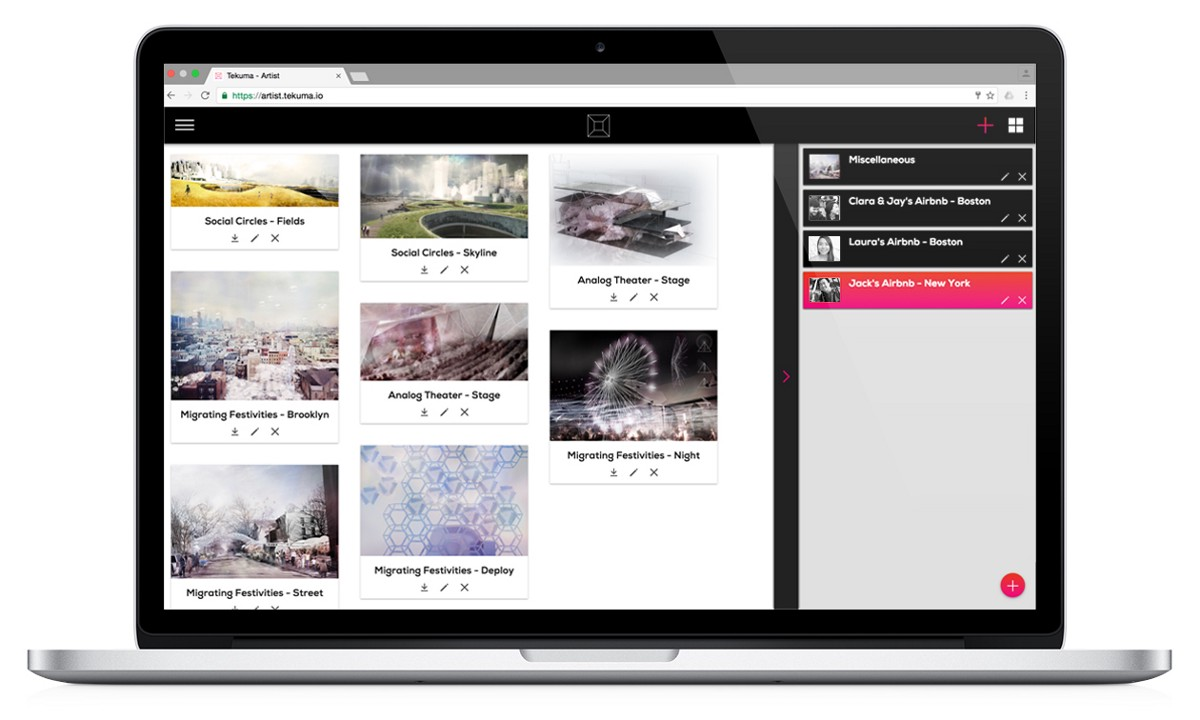
\includegraphics[scale=0.2]{./img/artist.jpg}
    \caption{The Artist Portal}
    \label{}
\end{figure}
The first component designed and implemented was the beta version of the Artist portal. The Artist portal is powered primarily by Google Firebase, and was originally designed to function without server-side code as a staticly served interface. All communications from the portal to the rest of the curation system are handled through the Firebase Realtime Database. The Artist Portal provides two main functionalities to its users, as well as a standard interface for editing and supplying personal information about themselves and their artistic style.\\

\subsubsection{Artist Studio}
The primary goal of the portal is to handle uploaded and cataloging of artworks. All uploaded files are saved into Google Cloud Storage buckets, located at in the Cloud Console\footnote, and all data cataloged in hierarchical (non-structural) format in the Firebase Database. The organization of these files within the storage buckets is detailed further in url-schema.md in the Documentation repositiory\footnote{}. Later, functionality was added to do extra processing on uploaded artworks to provide more labeled data. This functionality exceeded the scope of client-side execution, and integrating HTTP communication to a server would incure a large overhead. Instead, a daemon running on a Google Compute Engine (GCE) cloud-hosted server handles this extra processing. Communication to the daemon is facilitated by Google Firebase’s real-time database where a first-in-first-out (FIFO) stack is used to keep track of jobs for the daemon to execute. The extra labeling includes gathering text tags and color palletes from the uploaded images using machine-vision technology, and is further explained in (X.X).


\subsubsection{Artist Gallery}

\subsection{Business}
\subsection{Curator}
server and daemon (modularity)

\subsubsection{Curator Search}
\subsubsection{Curator Manage}
\subsubsection{Curator Review}
(discuss daemon)
\subsection{Discover}


\section{Unfinished Components}
\subsection{Business}
\subsection{Discovery}
% databasing all sales, and logging buyer behavior for data mining

\section{Databases}
\subsection{Arist Database}
Branches of the firebase database.
Used to handle state of artist.tekuma.io interface

\subsection{Curator Database}
branches of the firebase database
Used to handle state of the curator.tekuma.io interface

\subsection{Tekuma Artwork DB}

\subsection{Art.com Database}
The Art.com Database, which is roughly 10MB, contains \textbf{2,311,390} rows of data, in structured SQL format. Examples of these rows are below.\\

\begin{lstlisting}[language=Python]
columns = [ 'SKU', 'ITEM_TITLE',  'ITEM_LONG_DESC',  'ARTISTNAME',    'ITEM_TYPE',  'IMAGE_URL',  'PRODUCT_URL', 'PRODUCT_TAXONOMY' ]
actual_row = [ '30742196502A',
  'Spurzheim Bust',
  'JOHANN KASPAR SPURZHEIM German phrenologist with his autograph',
  'H Corbould',
  'Photographic Print',
  'http://cache2.allpostersimages.com/MED/\\84\\8488\\5WQK300Z.jpg',
  'http://www.art.com/products/p30742196502-sa-i9032642/.htm?RFID=197560',
  'World Culture>European  Cultures>German Culture>>>>>>>' ]
\end{lstlisting}

\section{Related Work}
\begin{enumerate}
    \item\textbf{ArtFlip} ( https://www.artflip.com/product) A website very similar in UI and UX to the curator portal.
\end{enumerate}

\section{Potential Innovative Development Projects}



\end{document}
